\documentclass[tikz, border=0px]{standalone}
\usepackage{tikz}
\usetikzlibrary{shapes,arrows}

\tikzstyle{startstop} = [rectangle,rounded corners,minimum width=3cm,minimum height=1cm,align=center,draw=black, text width=2.5cm, fill=green!30]

\tikzstyle{therapy} = [trapezium, trapezium left angle =70, trapezium right angle=110, minimum width=2cm, minimum height = 1cm, centered,draw=black,align=center, text width=2cm, fill=orange!30]

\tikzstyle{decision} = [diamond, minimum width = 3cm, minimum height = 3cm, text centered, draw=black, text width = 2cm,align=center,fill=blue!30]

\tikzstyle{arrow} = [thick, ->, >=stealth]
\tikzstyle{doublearrow} = [<->, thick, >=stealth]

\begin{document}
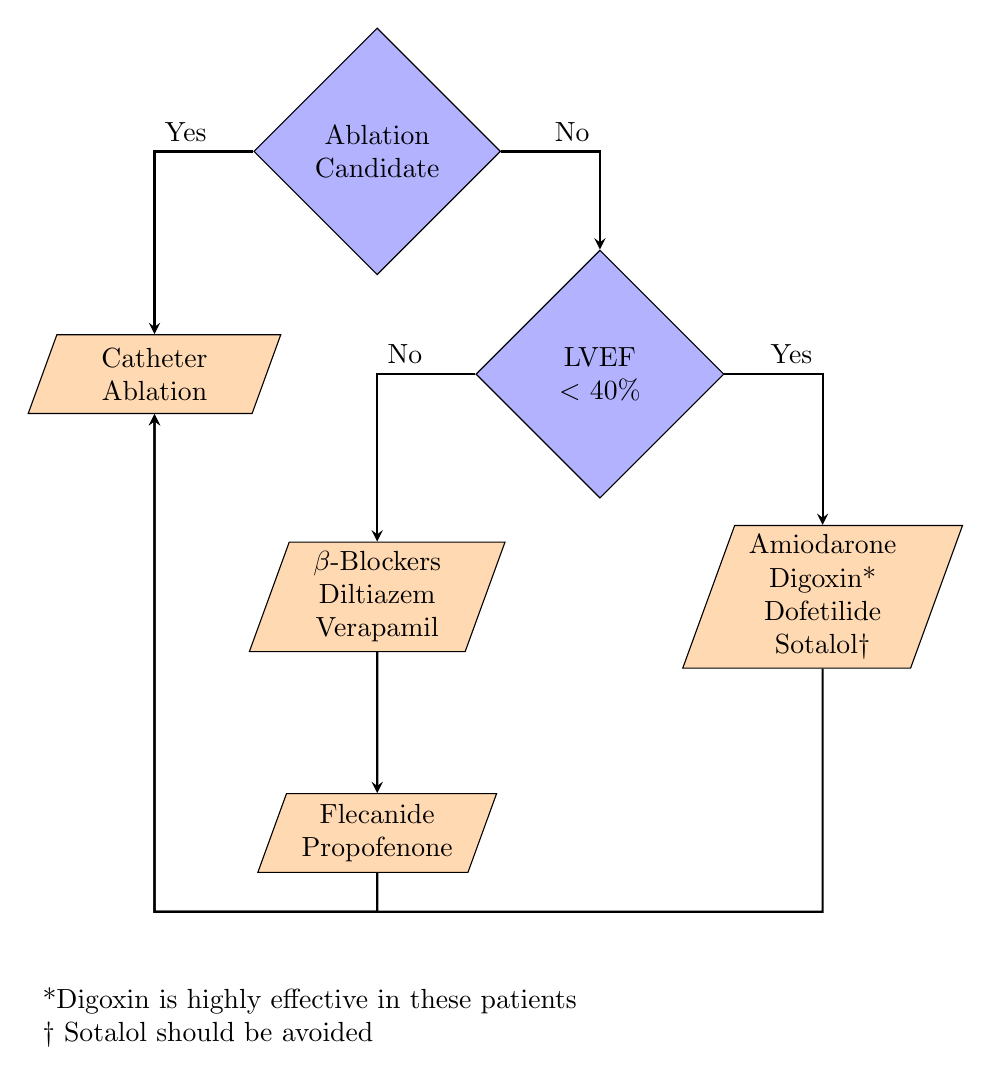
\begin{tikzpicture}[node distance=4cm]

\node (start) [decision] {Ablation Candidate};
\node (ablation) [therapy, below left of=start] {Catheter Ablation};
\node (comorbid) [decision, below right of=start] {LVEF $<$ 40\%};
\node (normal) [therapy, below left of=comorbid] {$\beta$-Blockers Diltiazem Verapamil};
\node (normalSecond) [therapy, below of=normal, yshift = 1cm] {Flecanide Propofenone};
\node (HFrEF) [therapy, below right of=comorbid] {Amiodarone Digoxin* Dofetilide Sotalol$\dagger$};

\node (notes) [rectangle, below of=start, yshift=-7cm, xshift=-0.75cm, text width = 7cm] {*Digoxin is highly effective in these patients\\ $\dagger$ Sotalol should be avoided};

\draw [arrow] (start) -| node[anchor=south west] {Yes} (ablation);
\draw [arrow] (start) -| node[anchor=south east] {No} (comorbid);
\draw [arrow] (comorbid) -| node[anchor=south east] {Yes} (HFrEF);
\draw [arrow] (comorbid) -| node[anchor=south west] {No} (normal);
\draw [arrow] (normal) -- (normalSecond);
\draw [arrow] (normalSecond) -- ++ (0,-1cm) -| (ablation);
\draw [arrow] (HFrEF) -- ++ (0,-4cm) -| (ablation);

\end{tikzpicture}
\end{document}